\section*{NAIL062 P\&P Logic: Worksheet 10 -- Resolution in predicate logic}
% after Lecture 10


\subsection*{Teaching goals:} After completing, the student

    \begin{itemize}\setlength{\itemsep}{0pt}
        \item understands the notion of unification and can perform the Unification Algorithm
        \item knows the necessary notions from the resolution method in predicate logic (resolution rule, resolvent, resolution proof/refutation, resolution tree), can formally define them, give examples, and explain the differences compared to propositional logic
        \item can apply the resolution method to solve a given problem (word problem, etc.), performing all necessary steps (conversion to PNF, Skolemization, conversion to CNF)
        \item can construct a resolution refutation of a given (possibly infinite) CNF formula (if it exists), can draw the resolution tree including the unifications used
        \item can extract an unsatisfiable conjunction of ground instances of axioms from a res. tree
        \item knows the notion of LI-resolution, can find an LI-refutation of a given theory (if exists)
        \item has become familiar with selected notions from model theory
    \end{itemize}
    

\section*{In-class problems}


\begin{problem} 
    
    \emph{Every barber shaves all those who do not shave themselves. No barber shaves anyone who shaves themselves.} Formalize and prove by resolution that: \emph{There are no barbers.}

    \begin{solution}

        First, we choose a suitable language. In the text we identify a property of objects ``$x$ is a barber'' and a relation between two objects ``$x$ shaves $y$''. We use the language $L=\langle B, S\rangle$ without equality, where $B$ is a unary relational symbol, $B(x)$ means ``$x$ is a barber'', $S$ is a binary relational symbol, $S(x,y)$ means ``$x$ shaves $y$''. 
        
        In this language we formalize the statements from the problem:
        \begin{itemize}
            \item Every barber shaves all those who do not shave themselves: 
            $$
            \varphi_1\ =\ (\forall x)(B(x)\limplies (\forall y)(\neg S(y,y)\limplies S(x,y)))
            $$
            \item No barber shaves anyone who shaves themselves: 
            $$
            \varphi_2\ =\ \neg (\exists x)(B(x) \land (\exists y)(S(x,y)\land S(y,y)))
            $$
            \item There are no barbers:
            $$
            \psi\ =\ \neg (\exists x)B(x)
            $$
        \end{itemize}
        Our goal is to show that in the theory $T=\{\varphi_1,\varphi_2\}$ the sentence $\psi$ is valid. We prove this by contradiction, starting with the theory $T\cup\{\neg\psi\}=\{\varphi_1,\varphi_2,\neg\psi\}$. Using Skolemization we obtain an equisatisfiable CNF formula $S$, then find its resolution refutation, showing that $S$ and hence $T\cup\{\neg\psi\}$ is unsatisfiable.

        Convert to PNF, Skolemize, remove universal quantifiers, and convert to CNF:
        \begin{itemize}
            \item $\varphi_1\ \rightsquigarrow\ B(x)\limplies (\neg S(y,y)\limplies S(x,y))\ \sim \ \neg B(x)\lor S(y,y)\lor S(x,y)$
            \item $\varphi_1\ \rightsquigarrow\ \neg(B(x)\land S(x,y)\land S(y,y))\ \sim\ \neg B(x)\lor \neg S(x,y)\lor \neg S(y,y)$
            \item $\neg\psi\rightsquigarrow\ B(c)$ (where $c$ is a new constant symbol)
        \end{itemize}
        Before starting Skolemization make sure you have sentences. And remember that we must Skolemize the sentence $\neg\psi$, not $\psi$. (The negation of a Skolem variant is typically not equisatisfiable with the negation of the original formula! By Skolemizing $\neg(\exists x)B(x)$ we would get $\neg B(x)$, whose negation is equivalent to $B(x)$, i.e.\ ``everyone is a barber'', whereas the correct procedure yields ``(a witness) $c$ is a barber''.)


        In set notation we have:
        $$
        S = \{\{\neg B(x), S(y,y), S(x,y)\},\{\neg B(x), \neg S(x,y), \neg S(y,y)\},\{B(c)\}\}
        $$
        Resolution refutation:
        \begin{align*}
            &\{B(c)\},\{\neg B(x), S(y,y), S(x,y)\},\{S(y,y),S(c,y)\},\{\neg B(x), \neg S(x,y'), \neg S(y',y')\},\\
            &\{\neg S(c,y'), \neg S(y',y')\},\square    
        \end{align*}
        The first two clauses are from $S$, the third is their resolvent using the unification $\{x/c\}$. The fourth clause is a variant of a clause from $S$, variable $y$ renamed to $y'$ to satisfy the technical condition of disjoint variable sets in resolved clauses. The fifth clause is the resolvent of the first and fourth clauses using unification $\{x/c\}$. The last, empty clause $\square$ is the resolvent of clauses 3 and 5 with unification $\{y/c,y'/c\}$.

        Typically, we represent the refutation as a resolution tree, indicating the unifications used:

        \begin{center}            
            \begin{forest}
                for tree={l=1.5cm, grow=north}
                [{$ \square $}, label=left:{\footnotesize\textcolor{blue}{$\{y/c,y'/c\}$}}
                    [{$ \{\neg S(c,y'), \neg S(y',y')\} $}, label=right:{\footnotesize\textcolor{blue}{$\{x/c\}$}}
                        [{$ \{\neg B(x), \neg S(x,y'), \neg S(y',y')\} $}]
                        [{$ \{B(c)\} $}]
                    ]
                    [{$ \{S(y,y),S(c,y)\} $}, label=left:{\footnotesize\textcolor{blue}{$\{x/c\}$}}
                        [{$ \{\neg B(x), S(y,y), S(x,y)\} $}]
                        [{$ \{B(c)\} $}]
                    ]
                ]
            \end{forest}
        \end{center}

    \end{solution}

\end{problem}


\begin{problem}

    The following statements describe a genetic experiment:
    \begin{enumerate}[(i)]\it
        \item Every sheep was either born from another sheep or cloned (but not both).
        \item No cloned sheep gave birth.
    \end{enumerate}
    We want to show by resolution that: {\it (iii) If a sheep gave birth, it was itself born.} Specifically:
    \begin{enumerate}[(a)]
        \item Express as sentences $\varphi_1$, $\varphi_2$, $\varphi_3$ in $L=\langle B,C\rangle$ without equality ($B$ is binary, $C$ unary relation symbol, $B(x,y)$ means `sheep $x$ gave birth to sheep $y$', $C(x)$ `sheep $x$ was cloned').
        \item Using Skolemization of these sentences or their negations, construct a set of clauses $S$ (possibly in an extended language) that is unsatisfiable exactly when $\{\varphi_1, \varphi_2\} \models \varphi_3$.
        \item Find a resolution refutation of $S$, draw the resolution tree with unifications used.
        \item Does $S$ have an LI-refutation?
    \end{enumerate}

    \begin{solution}
        Note that all objects are sheep, so no predicate for `being a sheep' is needed. The procedure is similar to the previous example:
        \begin{enumerate}[(a)]
            \item There are several ways to formulate the formulas; if we try to follow the text as closely as possible we get, for example:
            \begin{align*}
                \varphi_1 &\ =\ (\forall x)(((\exists y)B(y,x)\lor C(x))\land \neg ((\exists z)B(z,x)\land C(x)))\\
                \varphi_2 &\ =\ \neg(\exists x)(C(x)\land (\exists y)B(x,y))\\
                \varphi_3 &\ =\ (\forall x)((\exists y)B(x,y)\limplies (\exists z)B(z,x))
            \end{align*}
            \item Start from the theory $\{\varphi_1,\varphi_2,\neg\varphi_3\}$ (proof by contradiction). Convert to PNF, Skolemize, remove universal quantifiers, convert to CNF, and write in set notation:
            \begin{itemize}
                \item $\varphi_1\ \sim\ (\forall x)(\exists y)(\forall z)((B(y,x)\lor C(x))\land \neg (B(z,x)\land C(x)))\ \rightsquigarrow\ (B(f(x),x)\lor C(x))\land \neg (B(z,x)\land C(x))\ \sim\ \{\{B(f(x),x), C(x)\},\{\neg B(z,x), \neg C(x)\}\}$
                \item $\varphi_2\ \sim\ (\forall x)(\forall y)\neg (C(x)\land B(x,y))\ \sim\ \{\{\neg C(x),\neg B(x,y)\}\}$
                \item $\neg\varphi_3\ \sim\ (\exists x)(\exists y)(\forall z)\neg(B(x,y)\limplies B(z,x))\ \rightsquigarrow\ \neg(B(c,d)\limplies B(z,c))\ \sim\ \{\{B(c,d)\},\{\neg B(z,c)\}\}$
            \end{itemize}
            $$
            S = \{\{B(f(x),x), C(x)\},\{\neg B(z,x), \neg C(x)\},\{\neg C(x),\neg B(x,y)\},\{B(c,d)\},\{\neg B(z,c)\}\}
            $$
            \item Resolution tree for $S\proves_R\square$:
            \begin{center}            
                \begin{forest}
                    for tree={l=1.5cm, grow=north}
                    [{$ \square $}, label=left:{\footnotesize\textcolor{blue}{$\{y/d\}$}}
                        [{$ \{B(c,d)\} $}]
                        [{$ \{\neg B(c,y)\} $}, label=left:{\footnotesize\textcolor{blue}{$\{x/c,z/f(c)\}$}}
                            [{$ \{\neg C(x),\neg B(x,y)\} $}]
                            [{$ \{C(c)\} $}, label=left:{\footnotesize\textcolor{blue}{$\{x/c,z/f(c)\}$}}
                                [{$ \{\neg B(z,c)\} $}]
                                [{$ \{B(f(x),x), C(x)\} $}]
                            ]
                        ]
                    ]                    
                \end{forest}
            \end{center}
            \item Yes, in (c) we managed to construct an LI-refutation. Even if we had not, existence of an LI-refutation follows from the completeness theorem of LI-resolution for Horn formulas; our CNF formula $S$ is Horn.
        \end{enumerate}
                    
    \end{solution}

\end{problem}


\begin{problem}

    Let $T=\{\neg(\exists x) R(x),\ (\exists x)(\forall y)(P(x,y)\to P(y,x)),\ (\forall x)((\exists y)(P(x,y)\wedge P(y,x))\to R(x)),\ (\forall x)(\exists y)P(x,y)\}$ be a theory in the language $L=\langle P,R\rangle$ without equality.

    \begin{enumerate}[(a)]
        \item Using Skolemization, find an open theory $T'$ equisatisfiable with $T$.
        \item Convert $T'$ to an equivalent theory $S$ in CNF. Write $S$ in set representation.
        \item Find a resolution refutation of $S$. Indicate the unification used at each step.
        \item Find an unsatisfiable conjunction of ground instances of clauses from $S$. {\it Hint: use the unifications from (c).}       
    \end{enumerate}

    \begin{solution}
        
        \begin{enumerate}[(a)]
            \item By Skolemization we get: 
            $$
            T'=\{\neg R(x),\ P(c,y)\to P(y,c),\ P(x,y)\land P(y,x)\to R(x),\ P(x,f(x))\}
            $$
            (Be careful with the third axiom: $(\exists y)$ in the antecedent of the implication changes to $(\forall y)$.)
            \item Easily convert to CNF: 
            $$
            S = \{\{\neg R(x)\},\{\neg P(c,y),P(y,c)\},\{\neg P(x,y),\neg P(y,x),R(x)\},\{P(x,f(x))\}\}
            $$
            \item Resolution tree for $S\proves_R\square$:
            \begin{center}            
                \begin{forest}
                    for tree={l=1.5cm, grow=north}
                    [{$ \square $}, label=left:{\footnotesize\textcolor{blue}{$\{x/c,y/f(c)\}$}}
                        [{$ \{P(x,f(x))\} $}]
                        [{$ \{\neg P(c,y)\} $}, label=left:{\footnotesize\textcolor{blue}{$\{x/c,y'/y\}$}}
                            [{$ \{\neg P(c,y'),P(y',c)\} $}]
                            [{$ \{\neg P(x,y),\neg P(y,x)\} $}, label=left:{\footnotesize\textcolor{blue}{$\{x'/x\}$}}
                                [{$ \{\neg P(x',y),\neg P(y,x'),R(x')\} $}]
                                [{$ \{\neg R(x)\} $}]
                            ]
                        ]
                    ]                    
                \end{forest}
            \end{center}
            (Note where we need to rename variables to ensure disjoint variable sets in resolved clauses.)
            \item To obtain the conjunction of ground instances of axioms we can use the constructed resolution refutation. For each leaf of the resolution tree that is labelled by a clause $C$ (up to renaming it is a clause from $S$), we apply to $C$, in order, all the unifications that occur on the path from that leaf to the root:
            \begin{itemize}
                \item $\neg R(x)\cdot \textcolor{blue}{\{x'/x\}}\cdot\textcolor{blue}{\{x/c,y'/y\}}\cdot\textcolor{blue}{\{x/c,y/f(c)\}}=\neg R(c)$
                \item $\neg P(x',y)\lor\neg P(y,x')\lor R(x')\cdot \textcolor{blue}{\{x'/x\}}\cdot\textcolor{blue}{\{x/c,y'/y\}}\cdot\textcolor{blue}{\{x/c,y/f(c)\}}=\neg P(c,f(c))\lor \neg P(f(c),c)\lor R(c)$
                \item $\neg P(c,y')\lor P(y',c)\cdot\textcolor{blue}{\{x/c,y'/y\}}\cdot\textcolor{blue}{\{x/c,y/f(c)\}}=\neg P(c,f(c))\lor P(f(c),c)$
                \item $P(x,f(x))\cdot\textcolor{blue}{\{x/c,y/f(c)\}}=P(c,f(c))$
            \end{itemize}

            If variables remain in some clauses, we substitute any constant term for them. Thus we obtain the unsatisfiable conjunction of ground instances of clauses from $S$:
            $$
            \neg R(c)\land (\neg P(c,f(c))\lor \neg P(f(c),c)\lor R(c))\land (\neg P(c,f(c))\lor P(f(c),c))\land P(c,f(c))
            $$
            Its resolution refutation ``at the propositional level'' has the same structure as the resolution refutation of $S$:
                              
            \begin{minipage}{0.6\textwidth}
                \scalebox{0.9}{
                \begin{forest}
                    for tree={l=1.5cm, grow=north}
                    [{$ \square $}
                        [{$ \{P(c,f(c))\} $}]
                        [{$ \{\neg P(c,f(c))\} $}
                            [{$ \{\neg P(c,f(c)),P(f(c),c)\} $}]
                            [{$ \{\neg P(c,f(c)),\neg P(f(c),c)\} $}
                                [{$ \{\neg P(c,f(c)),\neg P(f(c),c),R(c)\} $}]
                                [{$ \{\neg R(c)\} $}]
                            ]
                        ]
                    ]                    
                \end{forest}
                }
            \end{minipage}%
            \begin{minipage}{0.35\textwidth}
                \scalebox{0.8}{
                \begin{forest}
                    for tree={l=1.5cm, grow=north}
                    [{$ \square $}
                        [{$ \{q\} $}]
                        [{$ \{\neg q\} $}
                            [{$ \{\neg q,r\} $}]
                            [{$ \{\neg q,\neg r\} $}
                                [{$ \{\neg q,\neg r,p\} $}]
                                [{$ \{\neg p\} $}]
                            ]
                        ]
                    ]                    
                \end{forest}
                }
            \end{minipage} 
            If we wanted to have ground instances of axioms of the original theory $T$, we would have to check which axiom was used to obtain each clause and apply the same unifications to it:
            $$
            \neg R(c)\land (P(c,f(c))\to P(f(c),c))\land (P(c,f(c))\land P(f(c),c)\to R(c))\land P(c,f(c))
            $$


        \end{enumerate}

    \end{solution}

\end{problem}

        
\section*{Extra practice}


\begin{problem}
    Find a resolution refutation: 
    \begin{align*}
        S=\{
            &\{P(a,x,f(y)),P(a,z,f(h(b))),\neg Q(y,z)\},\
            \{\neg Q(h(b),w),H(w,a)\},\ 
            \{\neg H(v,a)\},\\
            &\{\neg P(a,w,f(h(b))),H(x,a)\},\
            \{P(a,u,f(h(u))),H(u,a),Q(h(b),b)\}            
        \}
    \end{align*}
\end{problem}


\begin{problem}

    Let $L=\langle <, a, b, c\rangle$ be without equality, where $a,b,c$ are constant symbols (`apples/bananas/cherries') and $x < y$ expresses {\it ``fruit $y$ is better than fruit $x$''}. We know:
    \begin{enumerate}[(i)]\it
        \item The relation ``being better'' is a strict partial order (irreflexive, asymmetric, transitive).
        \item Pears are better than apples.
    \end{enumerate}
    Prove by resolution: \emph{(iii) If cherries are better than bananas, then apples aren't better than cherries.}

    \begin{enumerate}[(a)]
    \item Express statements $(i)$, $(ii)$, $(iii)$ as open formulas in the language $L$.
    \item Using these formulas, find a CNF formula $S$ that is unsatisfiable exactly when $(i)$ and $(ii)$ imply $(iii)$. Write $S$ in set representation.
    \item Prove by resolution that $S$ is unsatisfiable. Illustrate the refutation with a resolution tree, indicate the unification used at each step. {\it Hint: 4 resolution steps are enough.}
    \item Find a conjunction of ground instances of axioms of $S$ that is unsatisfiable.
    \item Is $S$ refutable by LI-resolution?
    \end{enumerate}

\end{problem}


\begin{problem}

    Let $T=\{\varphi\}$ be in $L=\langle U, c \rangle$ with equality, where $U$ is unary relational and $c$ is a constant symbol, and $\varphi$ expresses \emph{``There are at least 5 elements for which $U(x)$ holds.''}
    \begin{enumerate}[(a)]
        \item Find two non-equivalent complete simple extensions of $T$.
        \item Is the theory $T$ openly axiomatizable? Give justification.
    \end{enumerate}

\end{problem}


\begin{problem}

    Let $T = \{U(x) \to U(f(x)), (\exists x)U(x), \neg (f(x) = x), \varphi\}$ be a theory in the language $L = \langle U, f \rangle$ with equality, where $U$ is a unary relational symbol, $f$ is a unary function symbol, and $\varphi$ expresses that ``there are at most 4 elements.''
    \begin{enumerate}[(a)]
        \item Is the theory $T$ an extension of the theory $S = \{ (\exists x)(\exists y)(\neg x = y \land U(x) \land U(y)), \varphi \}$ in the language $L' = \langle U \rangle$? Is it a conservative extension? Justify.
        \item Is the theory $T$ openly axiomatizable? Justify.    
    \end{enumerate}
\end{problem}


\begin{problem}

    Let $T=\{(\forall x)(\exists y) S(y)=x,\ S(x)=S(y)\to x=y\}$ be a theory in the language $L=\langle S\rangle$ with equality, where $S$ is a unary function symbol.
    \begin{enumerate}[(a)]
        \item Find an extension $T'$ of the theory $T$ by definition of a new unary function symbol $P$ such that $T' \models S(S(x))=y \leftrightarrow P(P(y))=x$.
        \item Is the theory $T'$ openly axiomatizable? Give justification.
    \end{enumerate}

\end{problem} 


\begin{problem}

    Let $T$ be an extension of the theory $DeLO^-$ (i.e., dense linear orders with a minimal element and without a maximal element) by a new axiom $c \le d$ in the language $L=\langle \le,c,d\rangle$ with equality, where $c$, $d$ are new constant symbols.
    \begin{enumerate}[(a)]
        \item Are $(\exists x)(x\le d \wedge x \ne d)$ and $(\forall x)(x \le d)$ valid / contradictory / independent in $T$?
        \item Write two non-equivalent complete simple extensions of the theory $T$.
    \end{enumerate}
    
\end{problem}


\begin{problem}

    Consider the following graph.
    \smallskip
    
    \begin{minipage}{.72\textwidth}
        \begin{enumerate}[(a)]
            \item Find all automorphisms.
            \item Which subsets of the set of vertices $V$ are definable? Give the defining formulas. {\it (Hint: Use (a).)}
            \item Which binary relations on $V$ are definable?
        \end{enumerate}
    \end{minipage}%
    \begin{minipage}{.28\textwidth}        
        \vspace{-12pt}\hspace{12pt}
        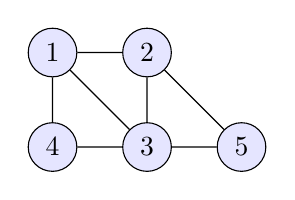
\begin{tikzpicture}[every node/.style={circle,fill=blue!10,draw,minimum size=0.5cm,node distance=1.2cm}]
            \node (1) {$1$};
            \node[right of=1] (2) {$2$};
            \node[below of=2] (3) {$3$};
            \node[left of=3] (4) {$4$};
            \path[draw] (1) -- (2) -- (3) -- (4) -- (1) -- (3);
            \node[right of=3] (5) {$5$};
            \path[draw] (2) -- (5) -- (3);
        \end{tikzpicture}        
    \end{minipage}%   

\end{problem}



\section*{For further thought}


\begin{problem}

    Let $T=\{(\forall x)(\exists y) S(y)=x,\ S(x)=S(y)\to x=y\}$ be a theory in the language $L=\langle S\rangle$ with equality, where $S$ is a unary function symbol.
    \begin{enumerate}[(a)]
        \item Let $\mathcal{R}=\langle\mathbb{R},S\rangle$, where $S(r)=r+1$ for $r\in\mathbb{R}$. For which $r\in\mathbb{R}$ is the set $\{r\}$ definable in $\mathcal{R}$ from the parameter $0$?
        \item Is the theory $T$ openly axiomatizable? Give justification.
        \item Is the extension $T'$ of $T$ by the axiom $S(x)=x$ an $\omega$-categorical theory? Is $T'$ complete?
        \item For which $0<n\in\mathbb{N}$ does there exist an $L$-structure $\mathcal{B}$ of size $n$ elementarily equivalent to $\mathcal{R}$? Does there exist a countable structure $\mathcal{B}$ elementarily equivalent to $\mathcal{R}$?
    \end{enumerate}

\end{problem}


\end{document}


